\documentclass[tikz,crop,convert={density=200,outext=.png},border=0.4cm]{standalone}

\usepackage{pgfplots}
\usepackage{amsmath}
\usetikzlibrary{arrows.meta}
\usepackage{physics}
\usepackage{xcolor}
\definecolor{mixed_1}{RGB}{2,56,88}
\definecolor{mixed_2}{RGB}{54,144,192}
\definecolor{mixed_3}{RGB}{208,209,230}
\pgfplotsset{compat=newest,
    %width=6cm,
    %height=3cm,
    scale only axis=true,
    max space between ticks=25pt,
    try min ticks=5,
    every axis/.style={
        axis y line=middle,
        axis x line=middle,
        axis line style={thick,->,>=latex, shorten >=-.3cm}
    },
    every axis plot/.append style={thick},
    tick style={black, thick},
}
\tikzset{
    semithick/.style={line width=0.8pt},
}
\usepgfplotslibrary{groupplots}
\usepgfplotslibrary{dateplot}
% Document begins
\begin{document}
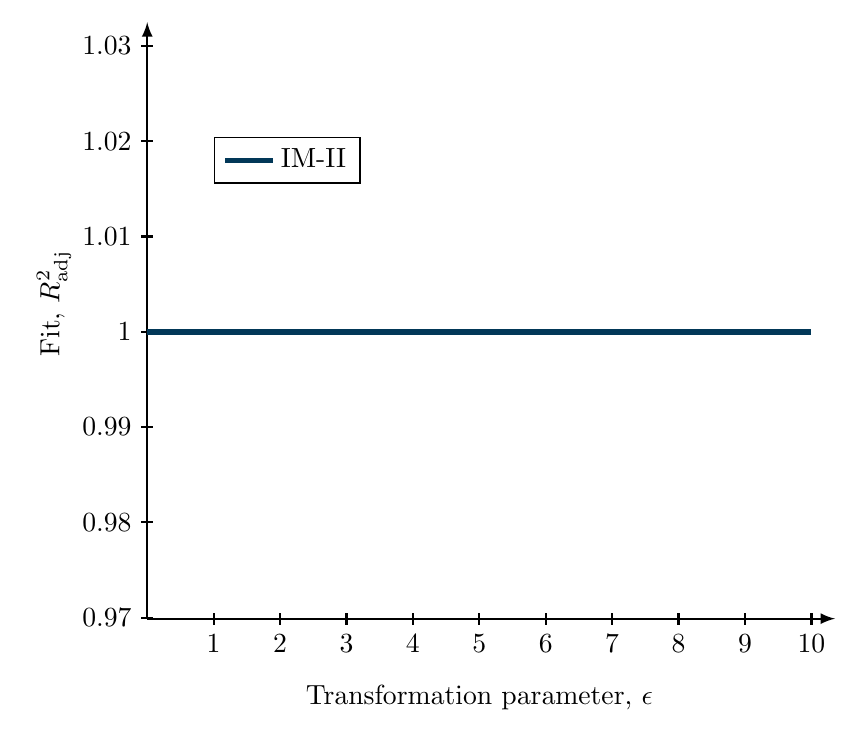
\begin{tikzpicture}
  % The axis of the plot
\begin{axis}[
    %title={Model: $\dv{y}{t}=\frac{2y}{t}$ with solution $y(t)=C_1t^2$\\Symmetry: $\Gamma_{\epsilon}=(t,y)\mapsto\left(\exp\left(\epsilon\right)t,\exp\left(-\epsilon\right)y\right)$},
    title style = {align=left},
    xlabel={Transformation parameter, $\epsilon$},
    % ylabel={The root mean square RMS, $\rho_0$},
    ylabel={Fit, $R^{2}_{\mathrm{adj}}$},
    %ylabel={Logarithm of Incidence, $\ln\left(R(t)\right)$},        
    x label style={at={(axis description cs:0.5,-0.1)},anchor=north},
    y label style={at={(axis description cs:-0.1,0.55)},rotate=90,anchor=south},    
    % xmin=0, xmax=82.5,
    %xmin=0, xmax=150.5,    
    % xmin=-27, xmax=5,
    ymin=0.9699, ymax=1.03,
    %xtick={-30,-27,...,9},
    %xtick={0,12,20,...,60,70,82},    
    %ytick={-15,-10,...,15},
    %legend style={at={(axis description cs:0.5,0.2)},anchor=west},
    %legend style={at={(axis description cs:0.1,1.2)},anchor=west},
    legend style={at={(axis description cs:0.1,0.8)},anchor=west},    
    %legend pos=north west,
    %ymajorgrids=true,
    grid style=dashed,
]
% Plot the model
\addplot[
color=mixed_1,line width=2pt,
]
coordinates {%
(0.0,1.0)
(0.10101010101010101,1.0)
(0.20202020202020202,1.0)
(0.30303030303030304,1.0)
(0.40404040404040403,1.0)
(0.5050505050505051,1.0)
(0.6060606060606061,1.0)
(0.7070707070707071,1.0)
(0.8080808080808081,1.0)
(0.9090909090909091,1.0)
(1.0101010101010102,1.0)
(1.1111111111111112,1.0)
(1.2121212121212122,1.0)
(1.3131313131313131,1.0)
(1.4141414141414141,1.0)
(1.5151515151515151,1.0)
(1.6161616161616161,1.0)
(1.7171717171717171,1.0)
(1.8181818181818181,1.0)
(1.9191919191919191,1.0)
(2.0202020202020203,1.0)
(2.121212121212121,1.0)
(2.2222222222222223,1.0)
(2.323232323232323,1.0)
(2.4242424242424243,1.0)
(2.525252525252525,1.0)
(2.6262626262626263,1.0)
(2.727272727272727,1.0)
(2.8282828282828283,1.0)
(2.929292929292929,1.0)
(3.0303030303030303,1.0)
(3.131313131313131,1.0)
(3.2323232323232323,1.0)
(3.3333333333333335,1.0)
(3.4343434343434343,1.0)
(3.5353535353535355,1.0)
(3.6363636363636362,1.0)
(3.7373737373737375,1.0)
(3.8383838383838382,1.0)
(3.9393939393939394,1.0)
(4.040404040404041,1.0)
(4.141414141414141,1.0)
(4.242424242424242,1.0)
(4.343434343434343,1.0)
(4.444444444444445,1.0)
(4.545454545454545,1.0)
(4.646464646464646,1.0)
(4.747474747474747,1.0)
(4.848484848484849,1.0)
(4.94949494949495,1.0)
(5.05050505050505,1.0)
(5.151515151515151,1.0)
(5.252525252525253,1.0)
(5.353535353535354,1.0)
(5.454545454545454,1.0)
(5.555555555555555,1.0)
(5.656565656565657,1.0)
(5.757575757575758,1.0)
(5.858585858585858,1.0)
(5.959595959595959,1.0)
(6.0606060606060606,1.0)
(6.161616161616162,1.0)
(6.262626262626262,1.0)
(6.363636363636363,1.0)
(6.4646464646464645,1.0)
(6.565656565656566,1.0)
(6.666666666666667,1.0)
(6.767676767676767,1.0)
(6.8686868686868685,1.0)
(6.96969696969697,1.0)
(7.070707070707071,1.0)
(7.171717171717171,1.0)
(7.2727272727272725,1.0)
(7.373737373737374,1.0)
(7.474747474747475,1.0)
(7.575757575757575,1.0)
(7.6767676767676765,1.0)
(7.777777777777778,1.0)
(7.878787878787879,1.0)
(7.979797979797979,1.0)
(8.080808080808081,1.0)
(8.181818181818182,1.0)
(8.282828282828282,1.0)
(8.383838383838384,1.0)
(8.484848484848484,1.0)
(8.585858585858587,1.0)
(8.686868686868687,1.0)
(8.787878787878787,1.0)
(8.88888888888889,1.0)
(8.98989898989899,1.0)
(9.09090909090909,1.0)
(9.191919191919192,1.0)
(9.292929292929292,1.0)
(9.393939393939394,1.0)
(9.494949494949495,1.0)
(9.595959595959595,1.0)
(9.696969696969697,1.0)
(9.797979797979798,1.0)
(9.8989898989899,1.0)
(10.0,1.0)
};
\addlegendentry{IM-II}

\end{axis}
\end{tikzpicture}

\end{document}
